\section{积分技巧}\label{020}

\subsection{换元 (substitution)}

事实上积分时的换元就是求导时的链式规则 (参见\ref{013}\nameref{013}) 反过来的过程.
具体操作是这样的, 例如若代求 \(\int f(x)\mathrm{d}x\), 有时为了计算方便,
我们 (i) 先定义另一个函数 \(u(x)\), 并利用 \(f(x)\) 和 \(u(x)\) 的关系,
将代积分的部分的 \(x\) 消去, 将其变为一个关于 \(u\) 的函数; (ii)
因为现在积分的对象不显含 \(x\) 了, 因此我们应该将最后的 \(\mathrm{d}x\)
也尝试变为 \(\mathrm{d}u\) (乘上一些项); 实际操作中 (i) 和 (ii)
步一般是同时进行的, 保证最后的形式是不显含 \(x\) 而只剩 \(u\); (iii)
最后, 若积分是一个定积分, 还要利用 \(x\) 和 \(u\) 的关系,
将积分上下限替换.

\begin{newquote}
例: 求 \(\int\sin^2(x)\cos(x)\mathrm{d}x\)

令: \(u=\sin(x)\)

则
\(\frac{\mathrm{d}u}{\mathrm{d}x}=\cos(x)\Rightarrow\mathrm{d}u=\cos(x)\mathrm{d}x\).

于是积分转化为 \(\int u^2\mathrm{d}u\), 后面的步骤便非常容易了.
\end{newquote}

\subsection{分部积分法 (integration by parts)}

分部积分法是由求导的乘法法则 (参见\ref{012}\nameref{012}) 而来, 求导的乘法法则有 \[
(fg)'(x)=f'(x)g(x)+f(x)g'(x),
\] 对其积分可以得到 \[
\int(fg)'(x)\mathrm{d}x=\int f'(x)g(x)\mathrm{d}x+\int f(x)g'(x)\mathrm{d}x,
\] 等式左边也可以写成
\(\int\frac{\mathrm{d}}{\mathrm{d}x}f(x)g(x)\mathrm{d}x\),
根据微积分基本定理, 积分和求导可以视作互为逆运算, 于是等式左边事实上便是
\(f(x)g(x)\), 挪项可得 \[
\int f(x)g'(x)\mathrm{d}x=f(x)g(x)-\int f'(x)g(x)\mathrm{d}x.
\] 更通常的, 很多教材会使用 \(u(x)\) 和 \(v(x)\), 省略 \((x)\),
分部积分法可以记作 \[
\boxed{\int u\ \mathrm{d}v=uv-\int \mathrm{d}u\ v}.
\]

\begin{newquote}
注意: 上式中的 \(\mathrm{d}\cdot\) 并不表示积分对象是 \(v\) 和 \(u\),
例如 \(\int u\mathrm{d}v\) 要表示的事实上还是
\(\int u(x)v'(x)\mathrm{d}x\); 另外 \(\int \mathrm{d}u\ v\) 中的 \(v\)
也是需要被积分的, 这么记事实上非常不规范.

物理和工程上经常很类似的, 会有 \(\int\mathrm{d}x f(x)\) 这样的写法,
没有把代积分的部分夹在积分符号和 \(\mathrm{d}x\) 之间, 而把
\(\mathrm{d}x\) 前置, 某种程度上是先强调了一下积分的对象是哪一个变量.
\end{newquote}

实际计算中,
分部积分法经常出现在对于【一个函数和三角函数或是指数函数的乘积】的积分,
下面是一个例子.

\begin{newquote}
例: \(\int x\cos x\ \mathrm{d}x\)

这个积分是用先前的知识是无法直接进行的, 遂用分部积分法; 首先要规定 \(u\)
和 \(\mathrm{d}v\), 然后求 \(\mathrm{d}u\) 和 \(v\);
用部分积分法的时候要尽可能的让 \(\int \mathrm{d}u\ v\) 这一项方便计算,
因此这一题中, 我们选取 \(u=x\), 这样一来
\(\mathrm{d}u=1\cdot\mathrm{d}x\) 就很方便接下来的计算;
所以便有\footnote{下面这个盒子是我高中的数学老师 Paul Elkin 传授的,
  他把它称作 ``working block'' (工作区),
  当然习惯了之后可以完全省略这个盒子里的内容, 但是初上手的时候,
  这样一个盒子可以很好地把关键步骤和''计算草稿''分割开来,
  使得书写面板很整洁, 也方便检查.}: \[
\boxed{\begin{aligned}
&u=x,&&\mathrm{d}v=\cos x\ \mathrm{d}x;\\
&\mathrm{d}u=\mathrm{d}x,&&v=\sin x.
\end{aligned}}
\] 于是 \[
\int x\cos x\ \mathrm{d}x=x\sin x-\int\sin x\ \mathrm{d}x.
\] 后续的计算因为不包含两个函数乘积的积分就很容易了.

类似的, 一个多项式乘以三角函数或是指数函数都可以用上述方法;
有时分部积分后得到新的积分项还是无法直接进行,
这时便需要继续对这一项使用分部积分, 使得多项式不断降次.

还有一些情况也可以使用分部积分, 例如 \(\int\ln x\ \mathrm{d}x\),
乍一看似乎看不出这个积分的结果, 一个提示是可以把 \(\ln x\) 视作
\(1\cdot\ln x\), 后续的计算留作练习.
\end{newquote}

一些超纲: 事实上, 部分积分法的思想不止局限于对函数的积分, 在变分法
(calculus of variation) 中, 在推导欧拉-拉格朗日方程 (Euler-Lagrange
equation) 时, 对泛函 (functional)\footnote{函数从映射的角度,
  是将数映射到数, 这里的''数''可能是实数, 也可能是虚数, 还可以是向量
  (什么是向量? 后面再细讲); 而泛函, 可以理解为函数的函数,
  泛函可以将函数映射到数, 它的定义域是函数构成的向量空间
  (什么是向量空间? 有机会再细说), 值域一般是实数.} 也可以有类似的操作
(翻出了我本科的毕业论文中的一段) :

\begin{figure}
\centering
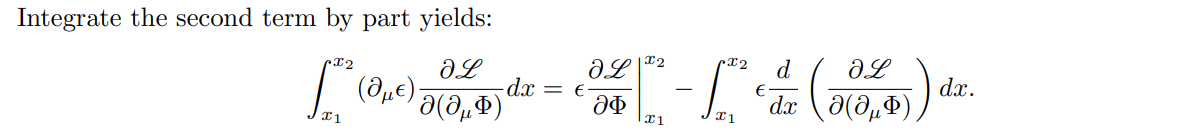
\includegraphics{image-20231101180718605.png}
\caption{image-20231101180718605}
\end{figure}

除此之外, 很多三角函数的积分可以利用三角函数的恒等式来化简;
两个多项式相除的积分可以利用部分分式 (partial fraction) 化简,
即将其变为若干个分式之和的形式; 更复杂的一些积分可以参考积分表,
作为一个现代人更可以合理使用一些计算软件辅助,
没有必要过分地去追求精通很多积分; 而且实际上,
很多积分并不能得到很好的解析式, 一般会用数值法来估算结果.
